\chapter{HW implementering og test}
%\section{Tryktransducer}
%Som tryktransducer anvendes TruWave (se datablad bilag). Herunder udregnes maksimalt udgangsspænding for tryktransducer ved maksimal trykbelastning (300 mmHg).
%\begin{align}
%V\lowercase{out} = 300 mmHg x 5 $\mu$ x 9V
%\end{align}



\section{Tryktransducer}
\subsubsection{Outputspænding} 
Vout = P * K * V+
\\
P = Tryk\\K = sensitivitet\\V+ = indgangsspænding\\ \\

Vmax = 300 mmHg * 5$\mu$ * 9 V\\
Vmax = 13,5 mV


\section{Operationsforstærker}
Som forstærkerblok anvendes INA 114. Denne har den fordel at gain kan kontrolleres af en variabel modstand (potentiometer). Forstærkningen skal være således at det maksimale input bliver forstærket til 5 V. 
\subsubsection{Forstærkning}
\begin{align}
G_{fblok} * 13,5 mV = 5 V\\
G_{fblok} = 370	
\end{align}

\subsubsection{Båndbredde}
På forstærkere generelt, og på INA 114, er produktet af båndbredden og forstærkningen en konstant. I vores tilfælde er dette 1.000.000.\\
Båndbredde ved gain på 370\\
1.000.000 = 370 * BW\\
BW = 2702 Hz > 50 Hz\\
Båndbredden er dermed bred nok til vores system.
\subsubsection{Gainmodstand}
Gainmodstanden er en modstand der bestemmer forstærkningen i INA 114.\\
\begin{align}
	G = 1+\frac{50k\Omega}{R_g}\\
	R_g = 135,4 \Omega
\end{align}

\section{Filterblok}
Som filter anvendes et Sallen Key lavpasfilter med unity gain.\\
Overføringsfunktion for filter\\
\begin{align}
	\frac{V_{out}(s)}{V_{in}(s)}=\frac{\frac{1}{R_1R_2C_1C_2}}{s^2+\frac{R_1+R_2}{R_1R_2C_2}+\frac{1}{R_1R_2C_1C_2}}
\end{align}
\subsubsection{Standardform}
\begin{align}
	\frac{V_{out}(s)}{V_{in}(s)}=\frac{w_n^2}{s^2+2\zeta\omega _n+w_n^2}
\end{align}
\begin{align}
	\omega _n = \sqrt{\frac{1}{R_1R_2C_1C_2}}
\end{align}
\\
Den ene kondensator, C2, sættes til 680nF (opgivet i opgaveformulering) mens den anden kondensator, C1, sættes til 340nF da denne er på lager. De to modstande sættes til samme værdi så: R = R1 = R2 
\begin{align}
	50*2\pi = \sqrt{\frac{1}{R^2*340*10^{-9}*680*10^{-9}}}
\end{align}
R isoleres og værdien findes\\ R = 6.620 k$\Omega$

\subsubsection{Magnitude Bodeplot}
\begin{figure}[H]
	\centering
	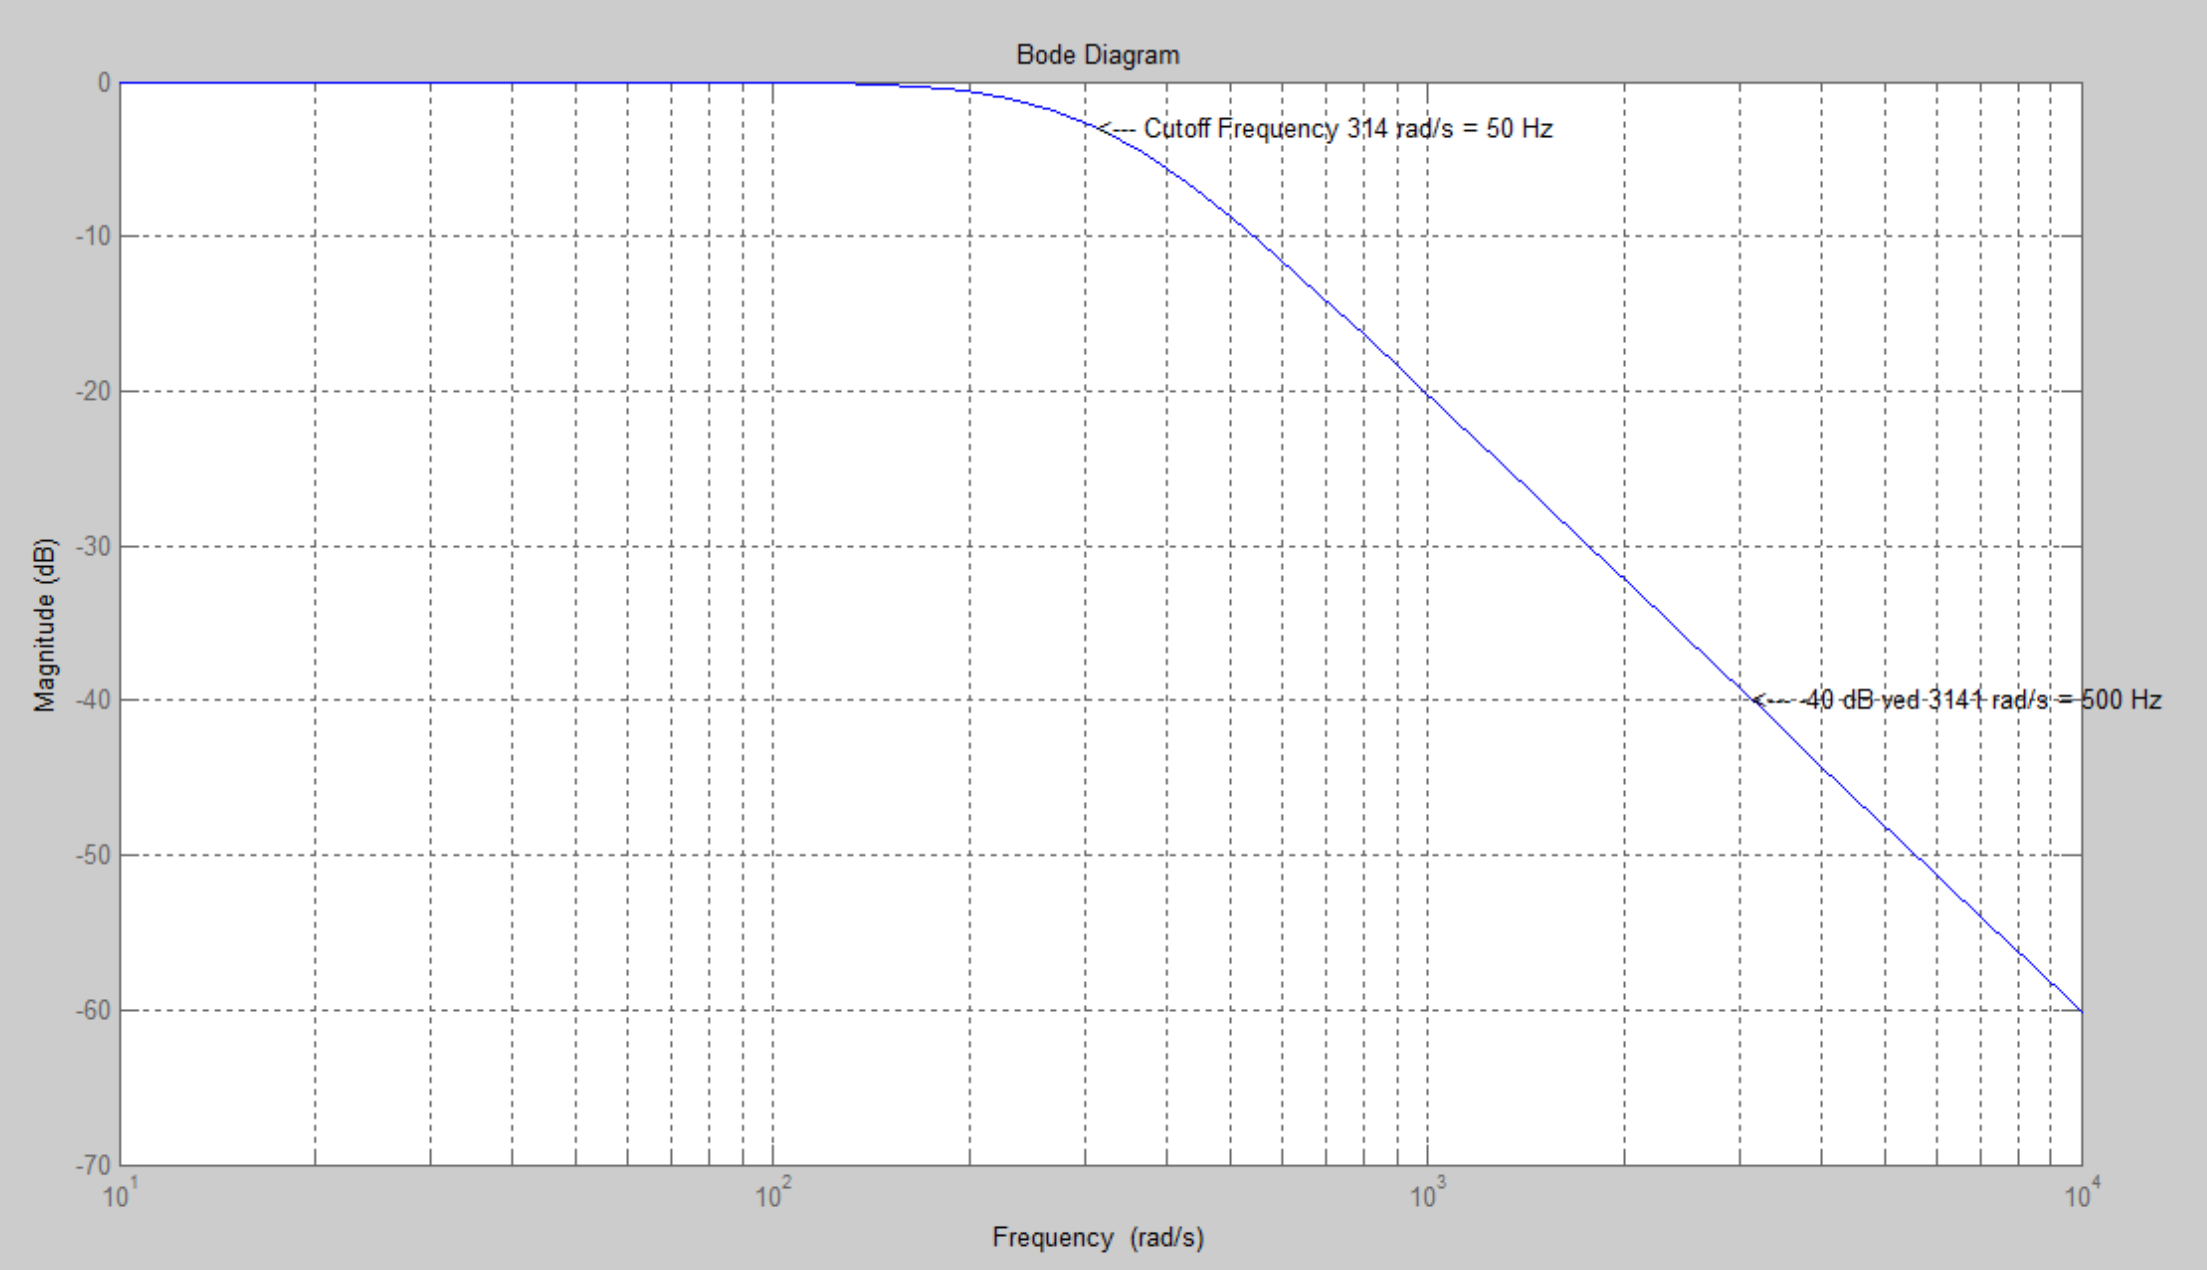
\includegraphics[width=1\textwidth]{Figurer/Bodeplot_Lavpasfilter_Teoretisk}
	\caption{Magnitude Bodeplot Lavpasfilter}
	\label{fig:Bodeplot}
\end{figure}

\subsubsection{Magnitude Bodeplot Beregning}
\begin{figure}[H]
	\centering
	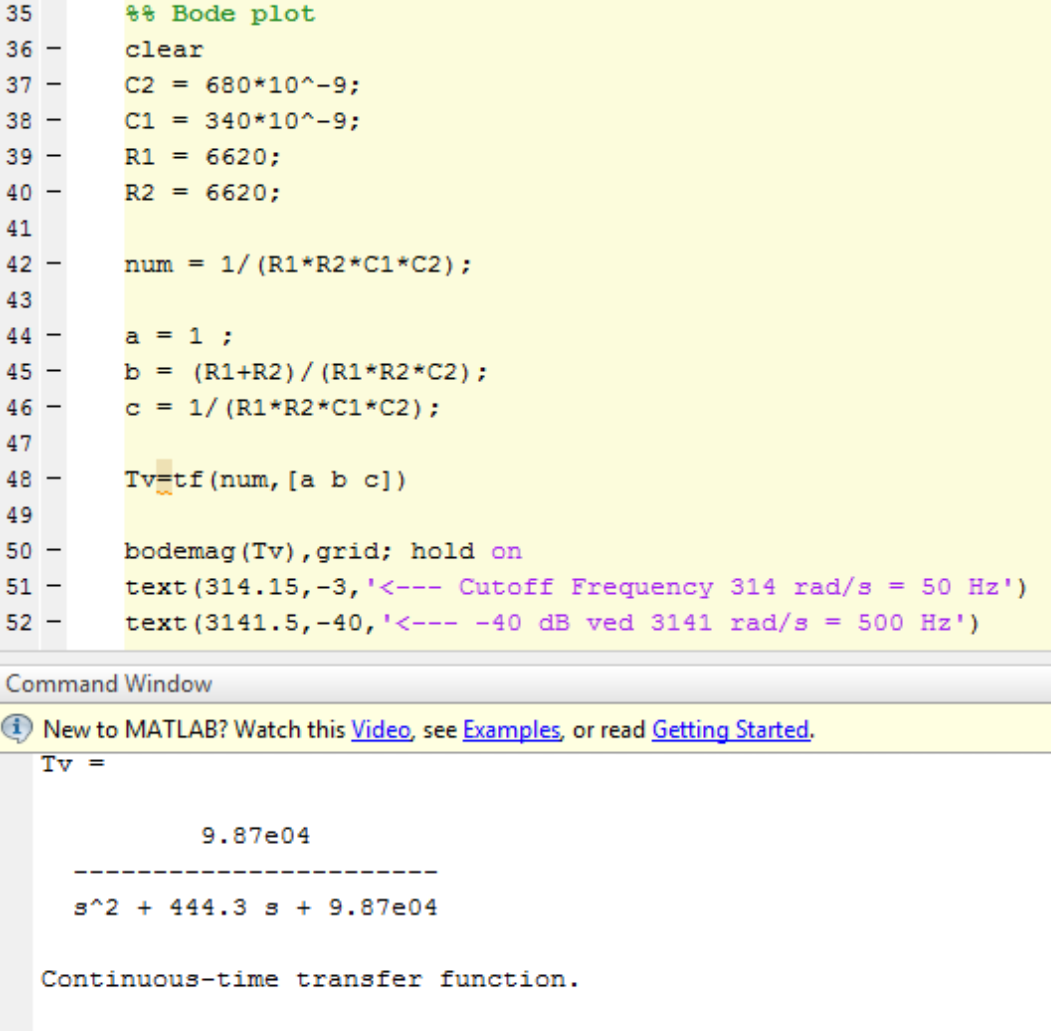
\includegraphics[width=0.5\textwidth]{Figurer/Beregninger_Bodeplot_teoretisk}
	\caption{Matlab Beregninger Bodeplot Lavpasfilter}
	\label{fig:Bodeplot Beregning}
\end{figure}


Følgende målinger er udført med komponentværdier, som i praksis gav bedre resultater end komponentværdierne udregnet i teori-afsnittet. Følgende komponenter er benyttet: 
R1 og R2: 2,3, C1: 340nF og C2: 680nF. 

Målingerne er foretaget ved at påsætte filteret en AC spænding på 5V med varierende frekvens i et spekter fra 1 Hz til 500 Hz. Dette gøres for at teste frekvensresponset på filteret. 

Channel 1 er indgangsspændingen og viser den varierende frekvens. Ændringen ses i venstre side af efterfølgende skærmbilleder. 
Oscilloskopet måler udgangsspændingen på filteret og resultatet vises i højre side af efterfølgende skærmbilleder. 

Følgende målinger er udført med komponentværdier, som i praksis gav bedre resultater end komponentværdierne udregnet i teori-afsnittet. Følgende komponenter er benyttet: 
R1 og R2: 2,3, C1: 340nF og C2: 680nF. 

Målingerne er foretaget ved at påsætte filteret en AC spænding på 5V med varierende frekvens i et spekter fra 1 Hz til 500 Hz. Dette gøres for at teste frekvensresponset på filteret. 

Channel 1 er indgangsspændingen og viser den varierende frekvens. Ændringen ses i venstre side af efterfølgende skærmbilleder. 
Oscilloskopet måler udgangsspændingen på filteret og resultatet vises i højre side af efterfølgende skærmbilleder. \\
Værdierne der gerne vil opnår er henholdsvis:


\begin{longtabu} to \linewidth{@{}l X[j]@{}}
	\textbf{Input} & \textbf{Output} \\[-1ex]
	\midrule
	5V 1Hz & 5V \\[-1ex]
	5V 50Hz	& 3.53V\\[-1ex]
	5V 500Hz & 0.5 V \\[-1ex]
	\caption{}	
\end{longtabu}

	

\begin{figure}[H]
	\centering
	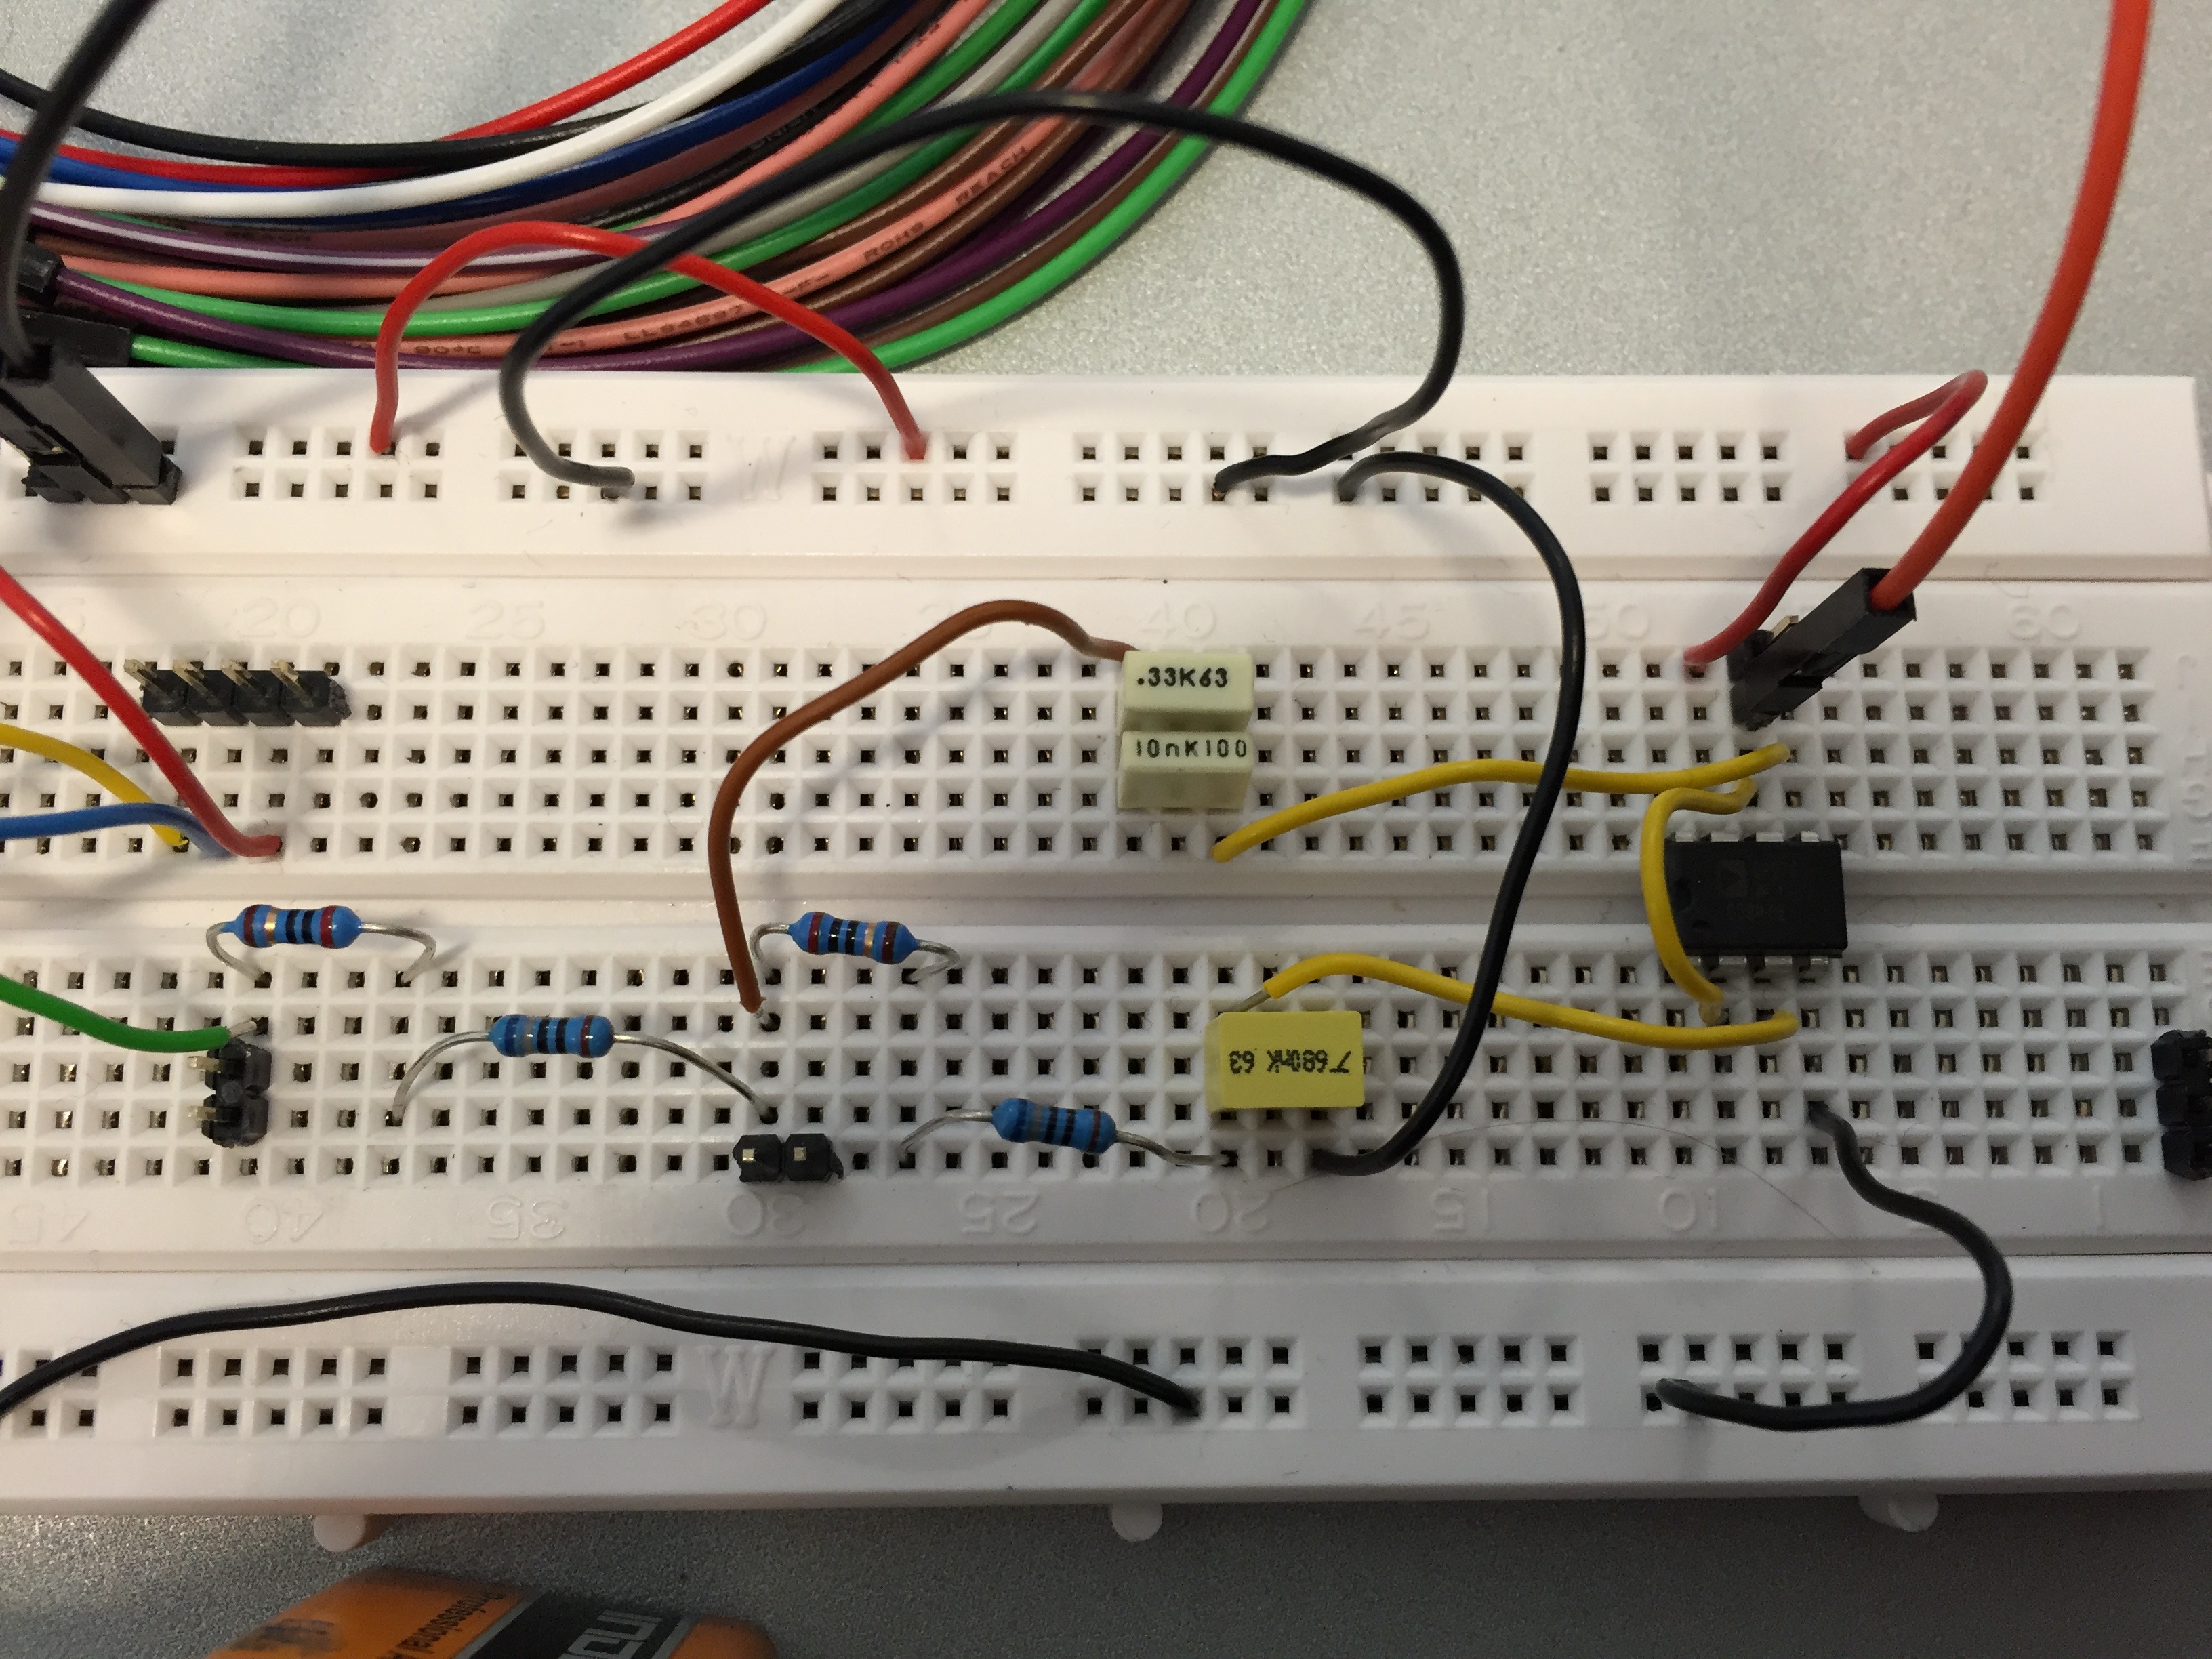
\includegraphics[width=1\textwidth]{Figurer/Filterblok}
	\caption{Praktisk opstilling af Filter}
	\label{fig:Filter}
\end{figure}

\begin{figure}[H]
	\centering
	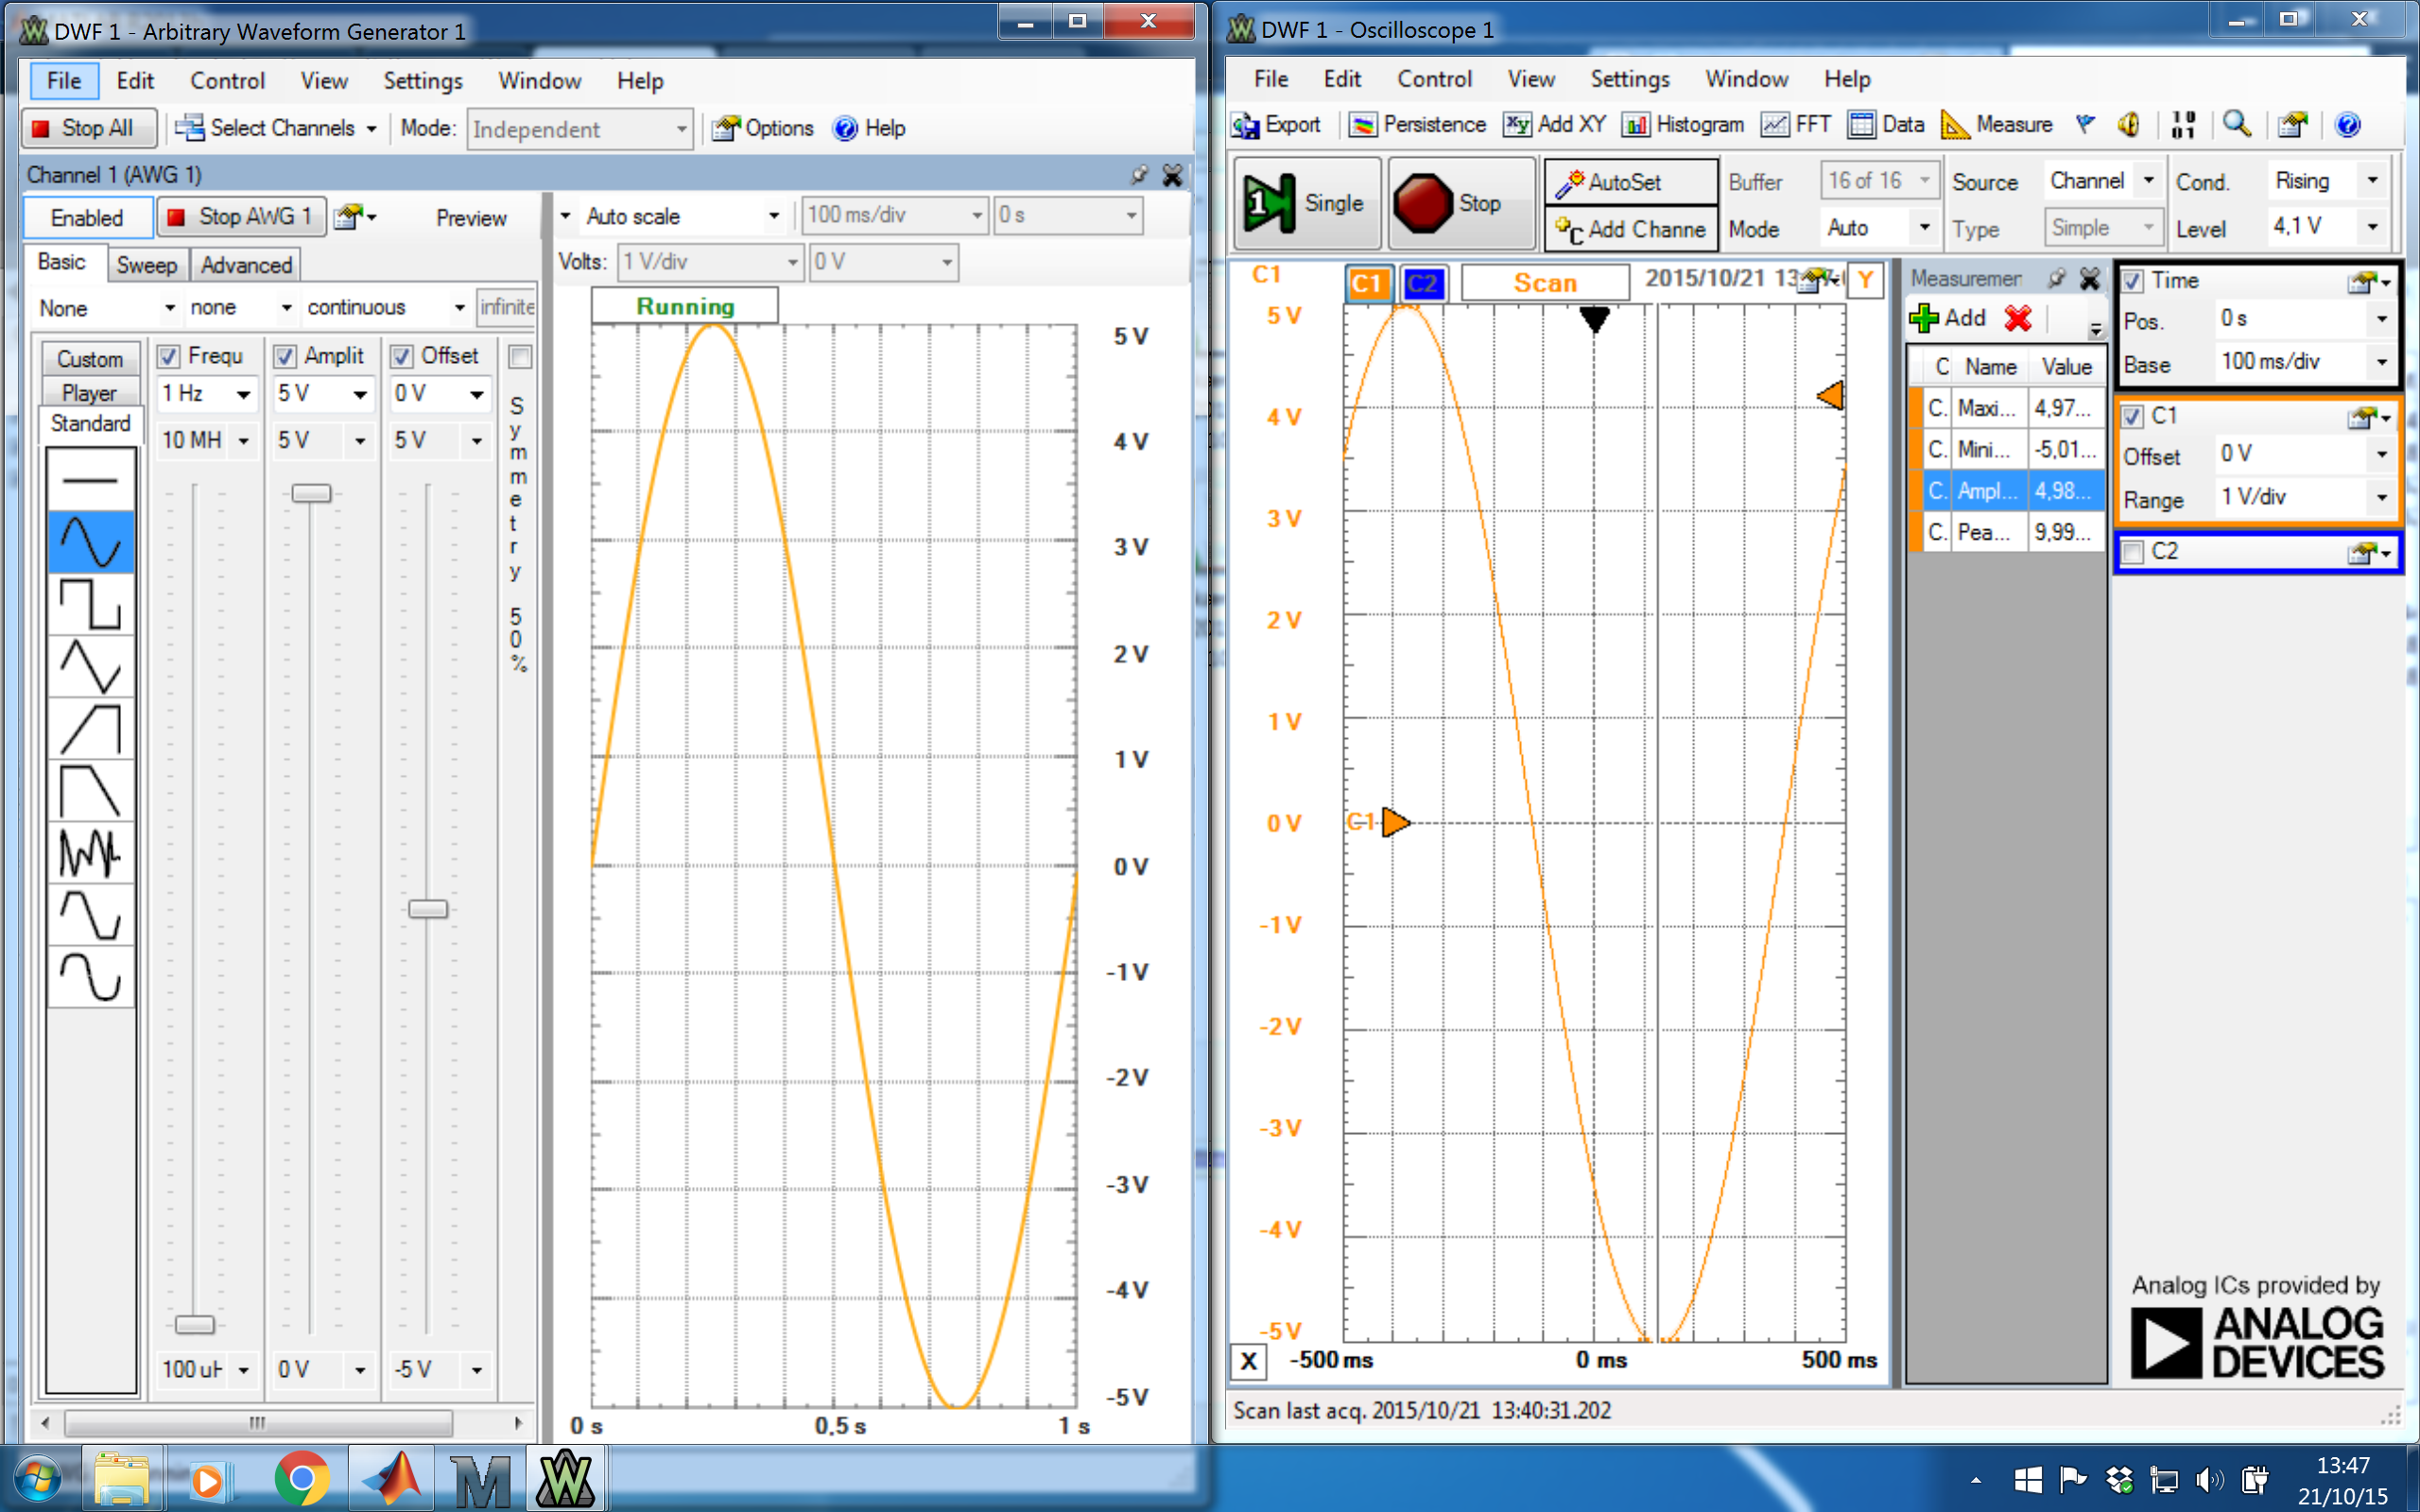
\includegraphics[width=1\textwidth]{Figurer/Lavpasfilter_Praktisk_1Hz}
	\caption{Lavpasfilter respons 1 Hz}
	\label{fig:Filter}
\end{figure}

\begin{figure}[H]
	\centering
	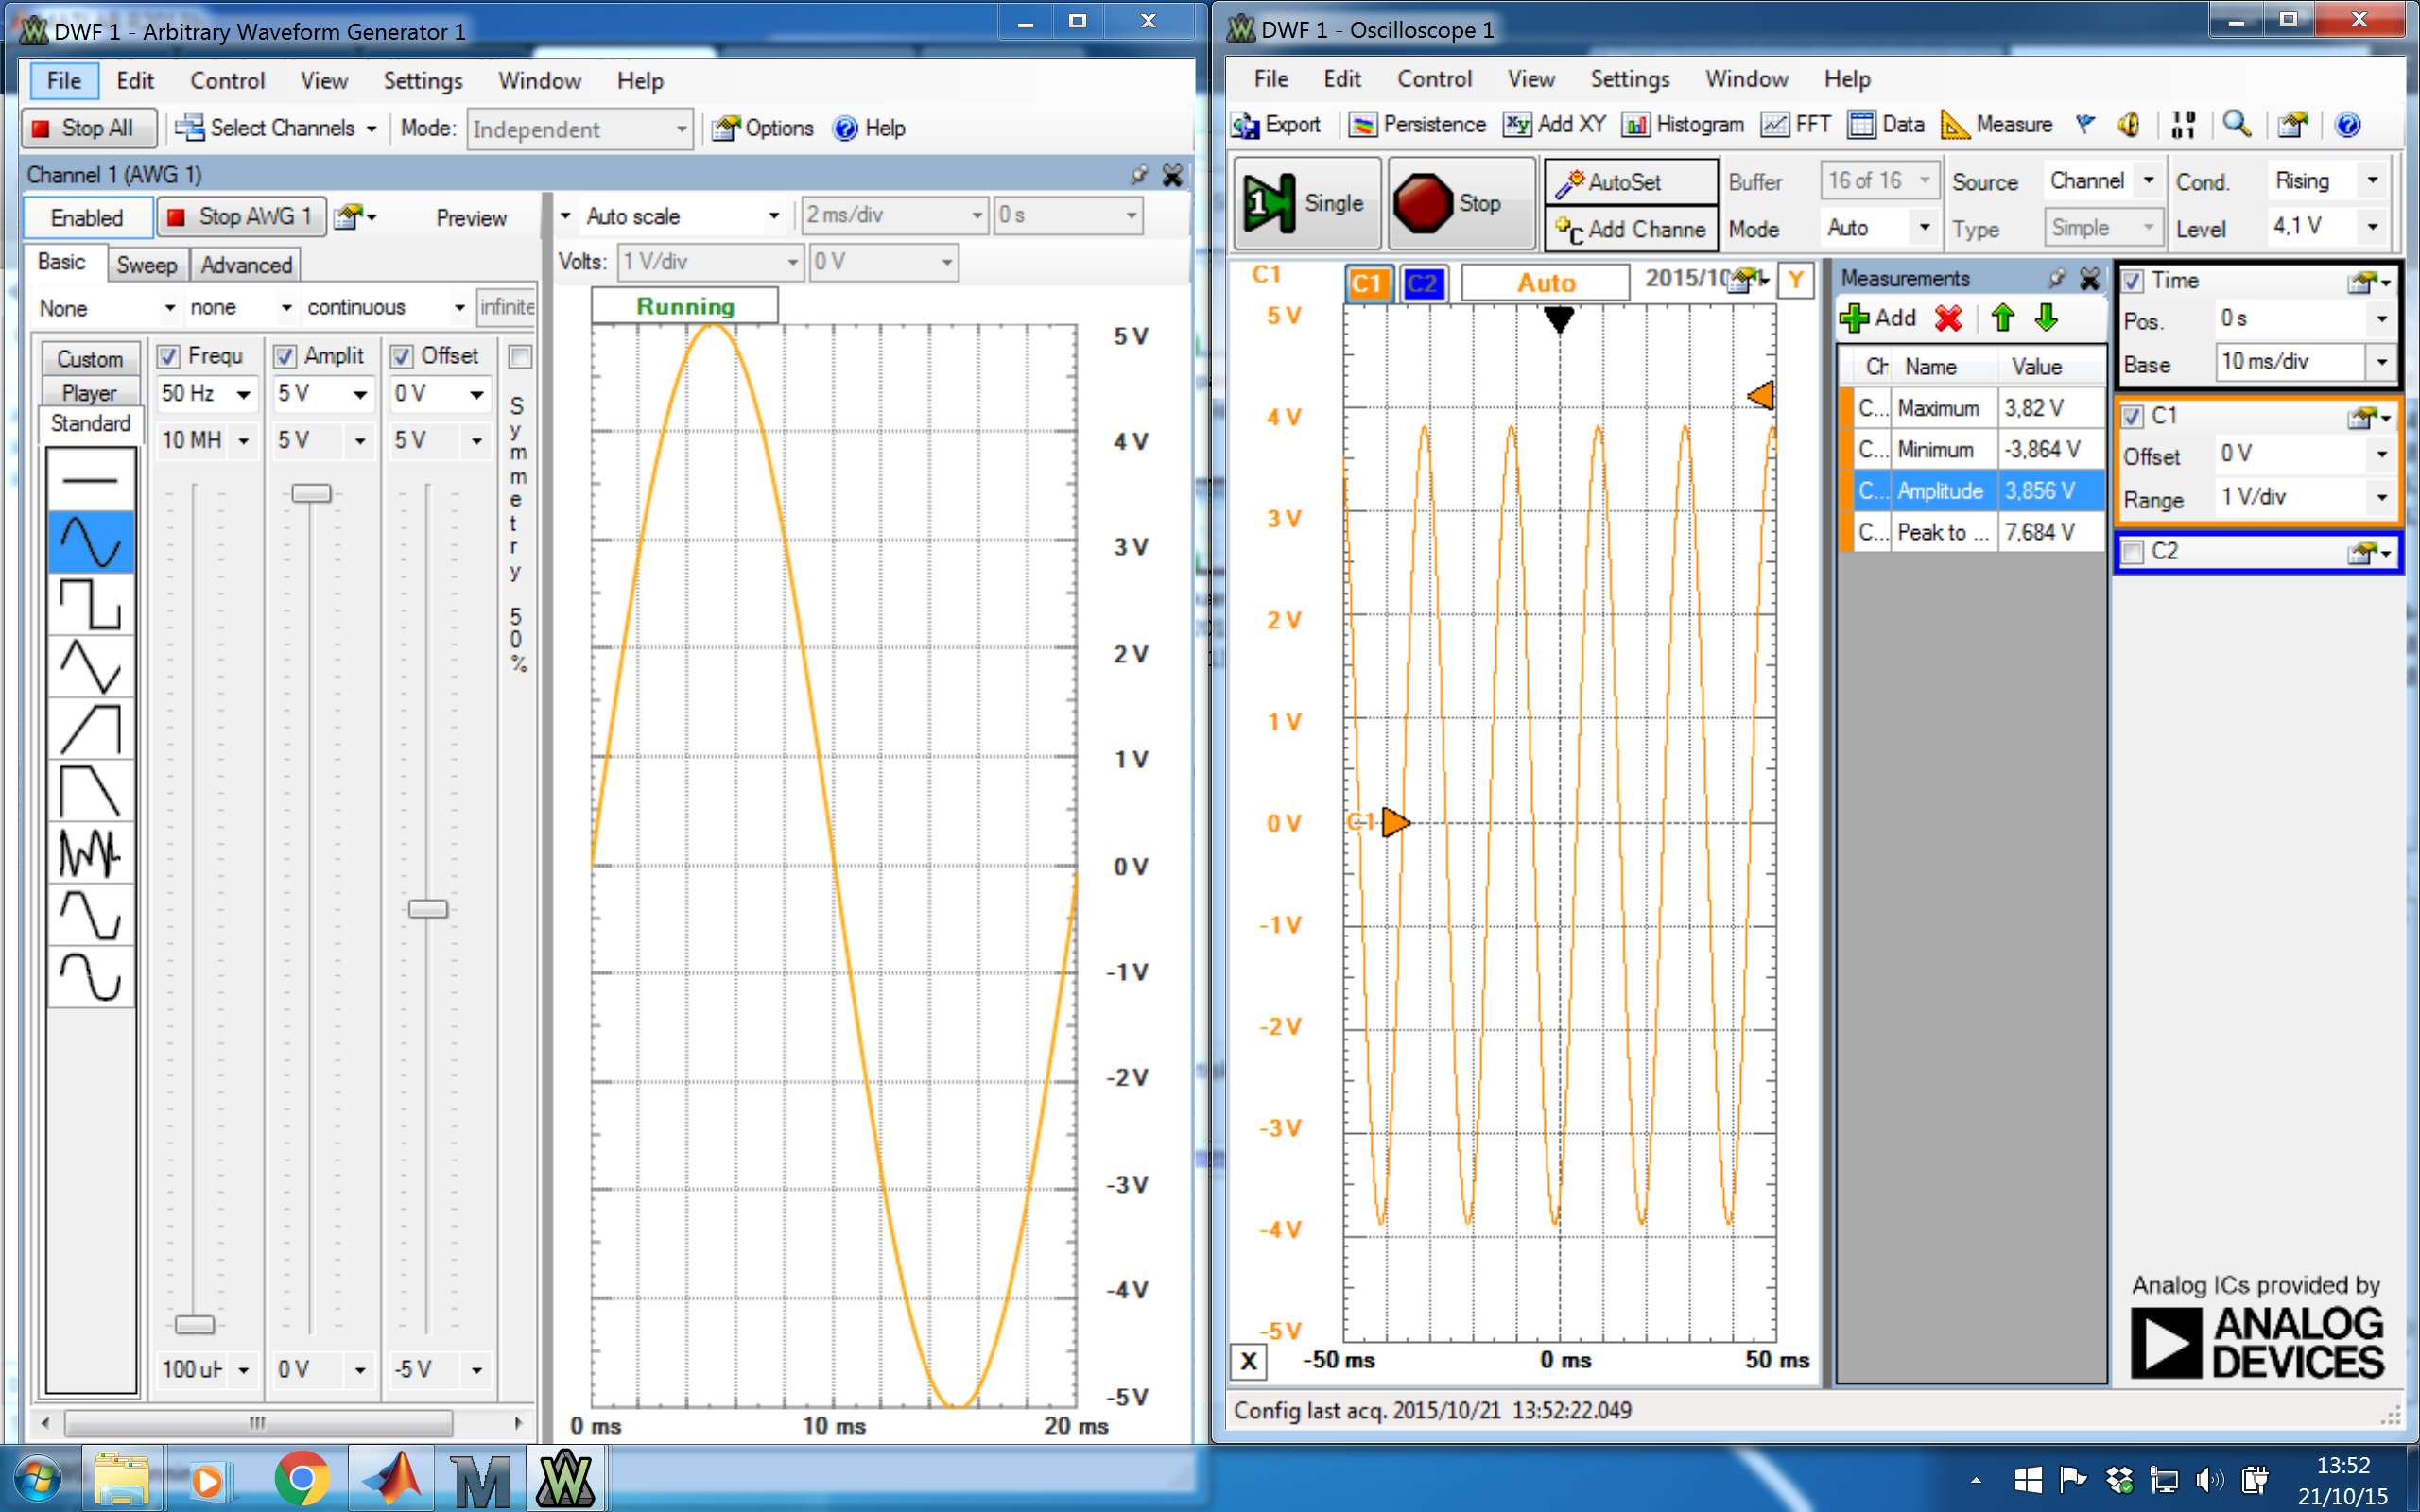
\includegraphics[width=1\textwidth]{Figurer/Lavpasfilter_Praktisk_50Hz}
	\caption{Lavpasfilter respons 50 Hz}
	\label{fig:Filter}
\end{figure}

\begin{figure}[H]
	\centering
	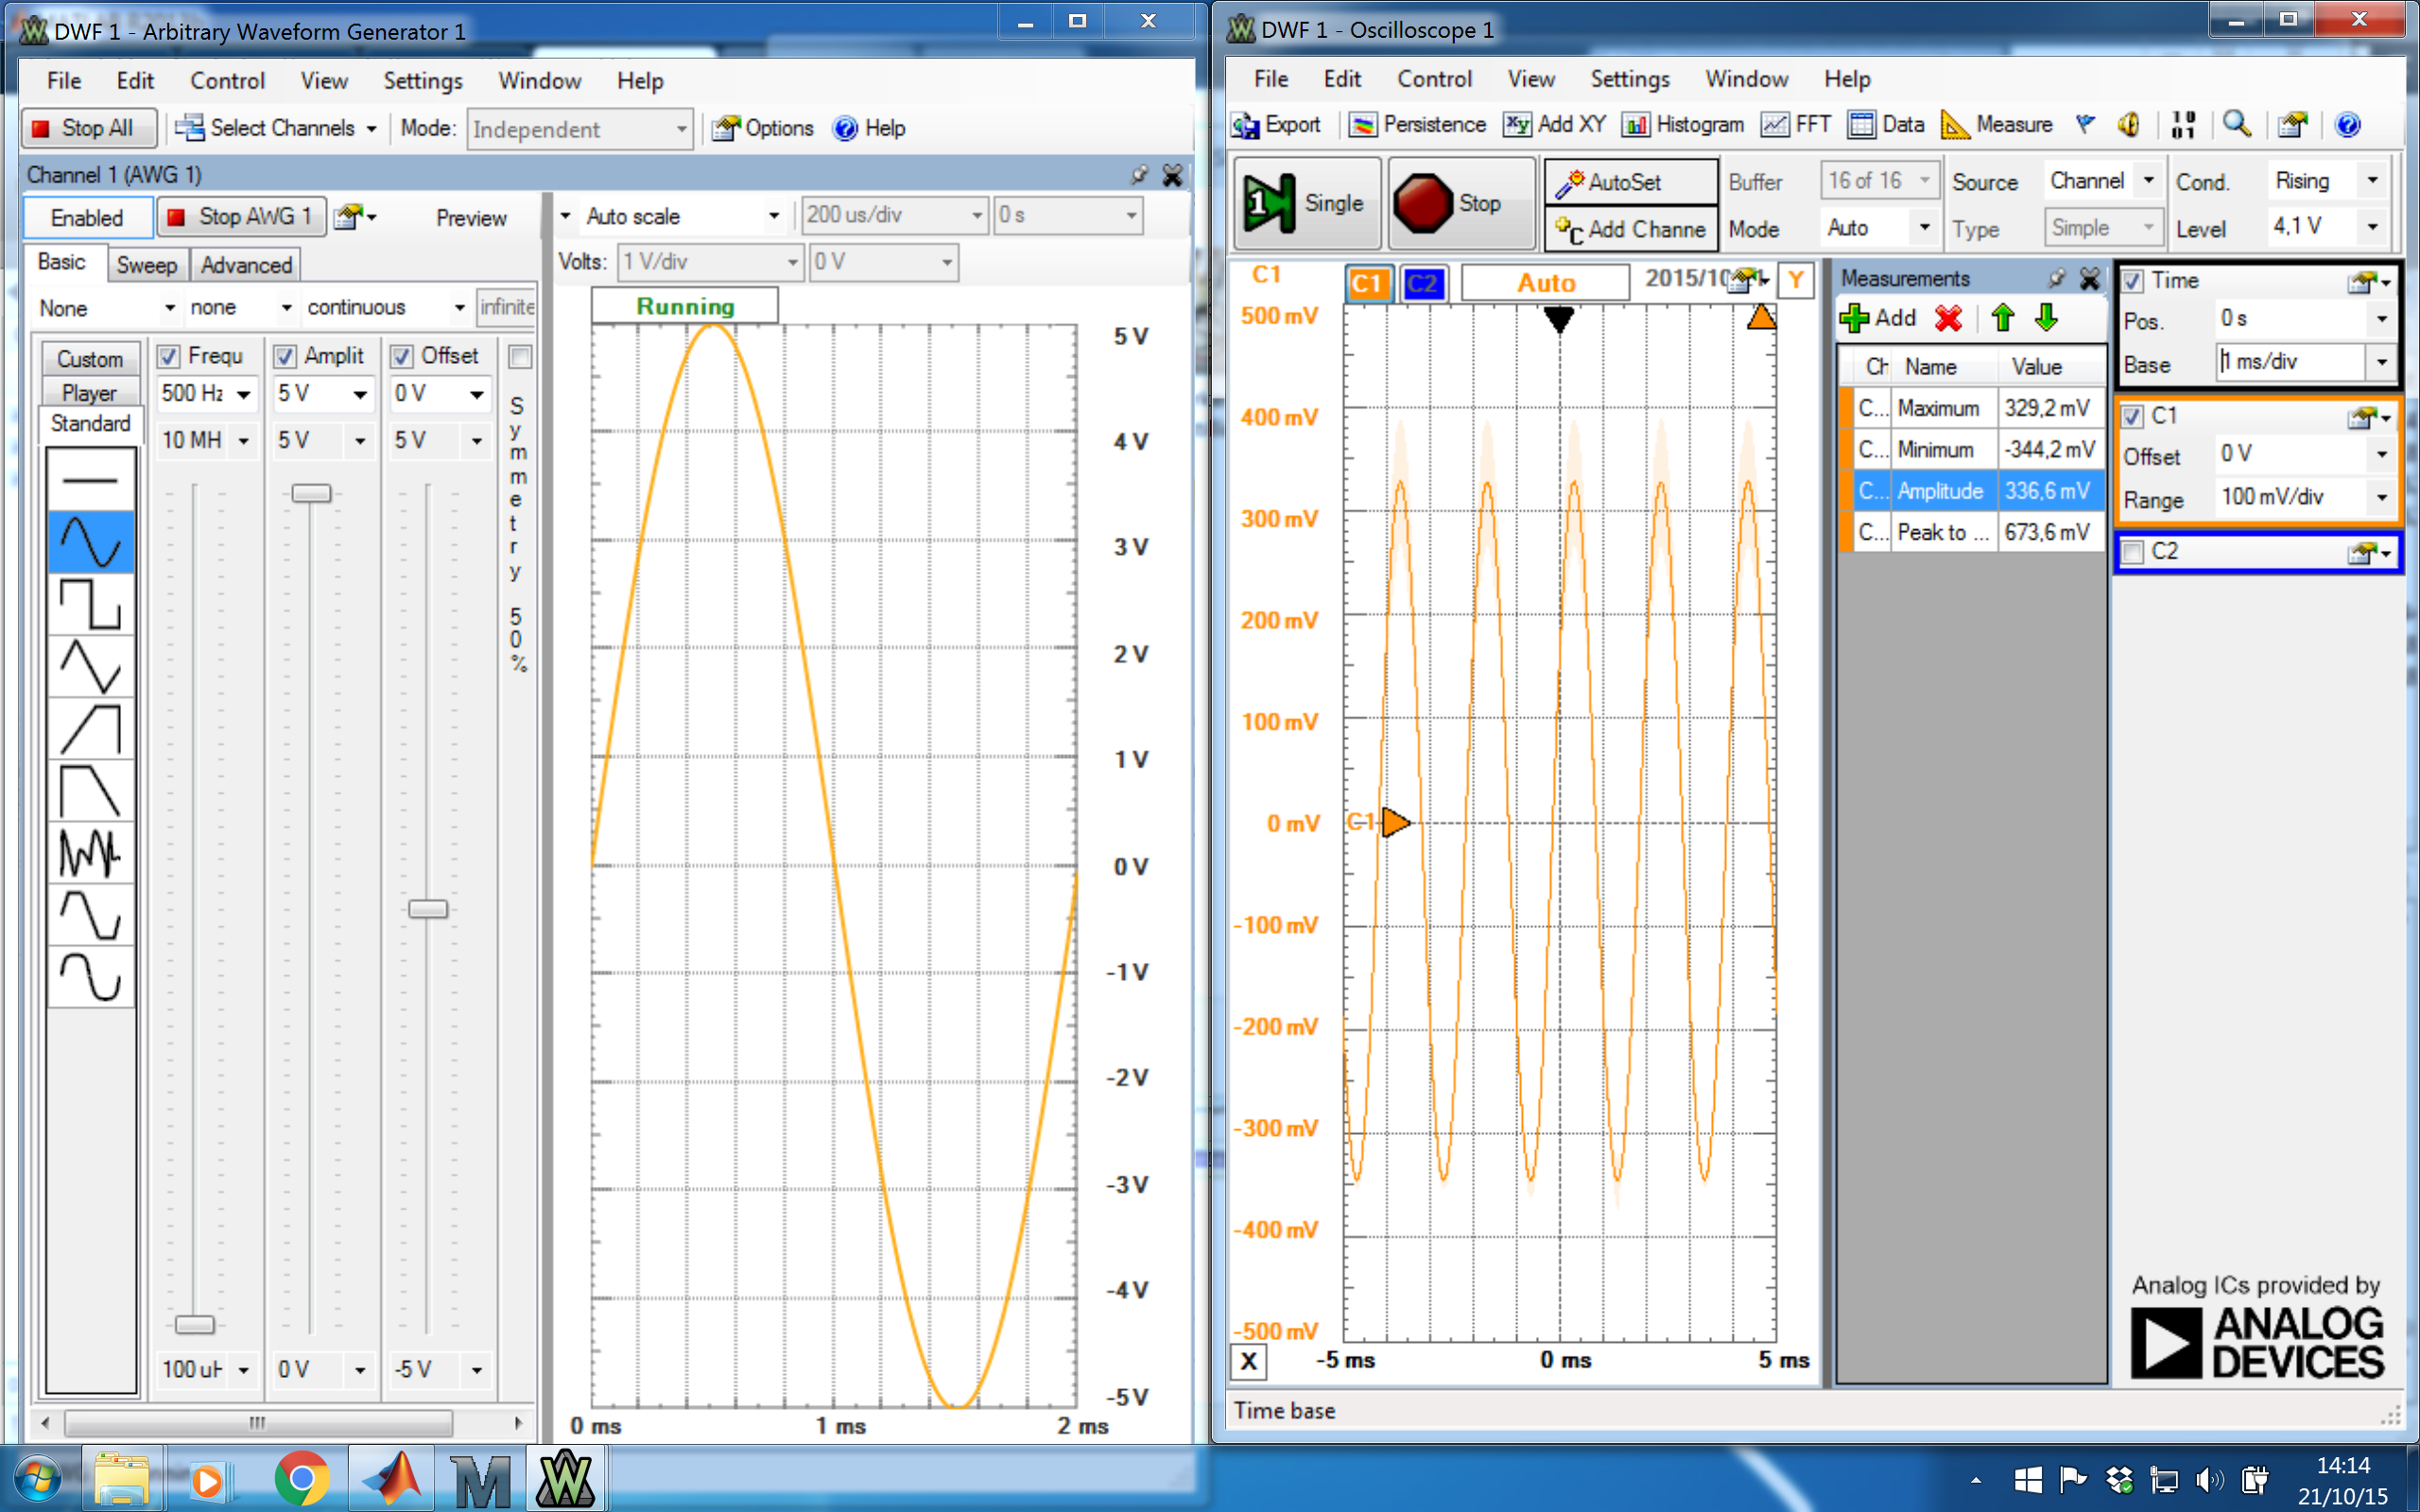
\includegraphics[width=1\textwidth]{Figurer/Lavpasfilter_Praktisk_500Hz}
	\caption{Lavpasfilter respons 500 Hz}
	\label{fig:Filter}
\end{figure}


